\documentclass{article}
\usepackage[utf8]{inputenc}
\usepackage{lstautogobble}
\usepackage[export]{adjustbox}
\usepackage{graphicx}
\usepackage{changepage}
\usepackage{listings}
\usepackage{amsthm}
\usepackage{subcaption}
\usepackage{amssymb}
\usepackage{titlesec}
\usepackage{hyperref}
\usepackage{lscape}
\usepackage{gensymb}

%Command to change name of table of contents
\renewcommand*\contentsname{Table of Contents}

%Command to start sections on new pages
\newcommand{\sectionbreak}{\clearpage}

%Create a new "Unlabeled section" that will be added to toc but not printed
\newcommand{\unlabeledsection}[1]{%
 \clearpage
  \par\refstepcounter{section}% Increase section counter
  \sectionmark{#1}% Add section mark (header)
  \addcontentsline{toc}{section}{\protect\numberline{\thesection}#1}% Add section to ToC
  }

\emergencystretch=1em

\title{OpenUAS:\\Fall 2020 Final Report }
\author{ }
\begin{document}


%%TITLE PAGE%%
\maketitle

\newpage

%%TEAM PAGE%%
\begin{center}
\Large \textbf{The OpenUAS Team}

\vspace{1cm}

\large{
 William Burken\footnote[1]{ISU Department of Mechanical Engineering}\\
 Ellie Diersen\footnote[2]{ISU Department of Aerospace Engineering}\\
 John Edgren\footnotemark[2]\\
 Chris Johannsen\footnote[3]{ISU Department of Electrical and Computer Engineering}\\
 Stephanie Jou\footnotemark[2]\\
 John Levandowski\footnotemark[2]\\
 Alex VandeLoo\footnotemark[2] \footnotemark[3]\\
 Adhyaksh Kumar\footnotemark[2]\\
 Colton Glick\footnotemark[3]\\
 Taylor Roquet\footnotemark[2]\\
 Camryn Medendorp\footnotemark[2]\\
 Marcella Anderson\footnotemark[3]\\
 Ashton Corpuz\footnotemark[1]\\
 Sara Mayne\footnotemark[1]\\
 Evelyn Moyer\footnotemark[2]\\
 Matthew Dodge\footnotemark[1]\\
}\par

\end{center}

\newpage

%%TABLE OF CONTENTS%%

\tableofcontents

%%PROJECT OVERVIEW%%
\section{Project Overview}

\subsection{Purpose}
Currently, there are no open-source unmanned aerial systems (UAS) which are fixed-wing and conceptually available to the general public. There are some similar UAS which are available to the public, but they must be purchased and are not open-source. The OpenUAS project is a multidisciplinary undergraduate research team aimed at developing an open-source fixed wing aircraft. The goal is to enable research teams, undergraduate/high school teams, and otherwise interested groups of people access to plans for a cheap, easy to manufacture, configurable fixed wing UAS to serve as an educational or test platform.\\\\
Dr. Kristin Rozier, assistant professor within Iowa State's Department of Aerospace Engineering, is the PI on the project. One of her main research areas is system health management for autonomous UAS. Therefore, one of the primary goals for this project is to act as a test bed for her research. As the UAS is also intended to be configurable, it is the end goal that the design can be used in additional research areas as well. Finally, the OpenUAS project is intended to be an educational module for advanced high school and college organizations.\\\\

\subsection{Scope}
In order to develop an open-source, COTS UAS for educational and research purposes that is free and available to the general public, a list of objectives, deliverables, and constraints were identified. The following section will provide an overview of these lists.

\subsection{Objectives}
\begin{enumerate}
\item Create an open-source, affordable, COTS UAS for educational and research flights
\item Provide full documentation of the conception, design, and testing of all systems
\item Act as a test bed for Dr. Rozier's system health management experiments
\item Be easily launched and not require a runway for takeoff or landing.
\item Be piloted by students and hobbyists
\item Be reconfigurable and support additional components
\end{enumerate}

\subsection{Deliverables}
\begin{enumerate}
\item A functioning design and prototype of a UAS
\item Relevant tools for piloting the UAS from the ground
\item Extensive documentation of the design process
\item Extensive documentation of the manufacturing process
\item Extensive documentation on proper use and safety
\item Extensive documentation on flight computer software and hardware options
\end{enumerate}

\subsection{Constraints}
\begin{enumerate}
\item COTS components
\item Affordable components
\item Reasonably duplicated components (e.g. all 3D printed parts can be reasonably produced by hobbyists)
\item All components should be reasonably safe (e.g. battery)
\end{enumerate}

%%RELATED WORK%%
\section{Related Work}
\noindent Currently, there are very few comparable fixed-wing UAS. The United States uses UAS such as the RQ-14A Dragon Eye and RQ-11B Raven in its military. Although these UAS are similar in size and weight to the OpenUAS team's target design, the technology and capabilities of these systems are much more advanced, and as such, the budget well exceeds the team's overall budget.\\

\noindent The University of Virginia created the Razor, a small fixed-wing UAS for the Department of Defense. This UAS has a flying wing design and utilizes an Android phone as the main processor. The Razor is of similar size, weight, and performance of the team's target design. One main difference in this system is that it is entirely 3D printed. The team plans on utilizing 3D printing, but not to the extent of the Razor design.\\

\noindent The Albatross is a commercial UAV produced by Applied Aeronautics. Although this aircraft is larger than the team's target design, its performance and low-cost are comparable to the team's goals. This UAV is described in more detail later in the paper, as the team purchased and is beginning to study this design. \\


%%STATUS%%
\section{General Information}

\subsection{Status}
For the Fall 2020 semester the OpenUAS team built and tested the second prototype of the OpenUAS. The prototype can be seen in \ref{fig:UAS_2.0_model} below. The testing that took place includes a standing thrust test as well as a full test flight which resulted in a successful flight but unfortunately not a successful landing. \\

In spite of the Covid-19 pandemic and the various restrictions put in place for safety, the team was able to construct the UAS over the course of semester. These challenges will be elaborated later on. Further, the design team was able to make incremental improvements to the design which was manufactured this semester. This improved design will be constructed in the following semester. The electronics/software team was able to improve upon the electronic system and test out various components through the flight test. including autonomous flight capabilities included with the flight controller.

\begin{figure}[hbt!]
\centering
\includegraphics[width=0.75\textwidth]{./Images/standing_thrust_test1.jpg}
\caption{Fall 2020 OpenUAS Prototype}
\label{fig:UAS_2.0_model}
\end{figure}

\subsection{Team Organization}
The flowchart \ref{fig:UAS_team_org} on the next page shows the organizational structure of the OpenUAS team.

\newpage

\begin{landscape}
\begin{figure}[hbt!]
\centering
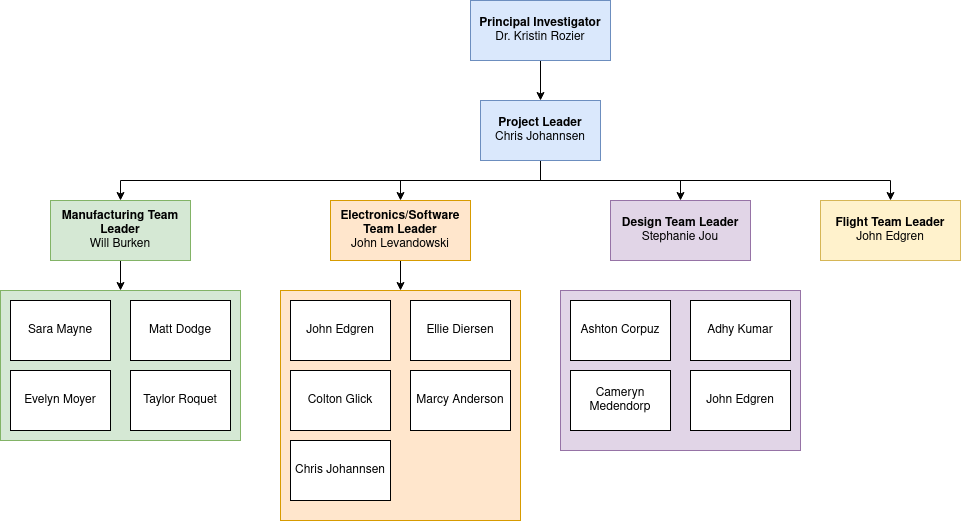
\includegraphics[scale=0.6]{Images/openuas_team_org.png}
\caption{Fall 2020 OpenUAS Team Organization}
\label{fig:UAS_team_org}
\end{figure}
\end{landscape}

\newpage

\subsection{Documentation}
Varying forms of documentation were developed to assist with tracking the vision, objectives, high-level project plan, and weekly progress and goals. The documentation is intended to not only support the systems engineering aspect of the project, but also serve an educational purpose by assisting future users who would like insight into what efforts and decisions were made to bring OpenUAS from a concept to a reality. Additionally, everyone on the team keeps their own weekly and semester progress documentation to maintain goals and the vision for every subgroup within the OpenUAS team. \\

\subsection{Lab Set-Up \& Organization}
The lab originally started out with no equipment or tools available for our project. Throughout the last school year, orders had been placed for tools and other items needed in order to ensure a work space that has all tools needed for successful progression of this project. This last semester has built off what was completed before, adding new equipment, rearranging tables and desks to provide more surface area in the lab for various projects, and adding more tool locations for easier access to common tools.  Because we are working within a large organization, special documentation and communication must be done in order to acquire the parts needed for the lab. This includes confirmation of successful retrieval of parts and checking if damage was done to them. If damage is found, proceeding with the proper return process and notifications so everyone knows how parts are moving about. If an item is not the item we purchased (e.g. a different sized cartridge for a label printer) we send it back to the individual keeping track of our orders and have them re-order the right equipment. The final goal is to have a lab outfitted in such a way that it can complete any of the tasks designed for the project with exceptions to precision machining and other similar processes.

%%INSPIRATION: THE ALBATROSS%%
\section{Primary Inspiration: The Albatross UAV}
The Albatross UAV is a commercial product of Applied Aeronautics. The team purchased this model in the fall of 2017 to study the documentation, the ease of construction, and the flight characteristics of this model. The Albatross UAV has a wingspan of approximately 9.8 feet and is advertised to carry over 4.4 kg of payload over 4 hours. The Albatross is capable of a maximum 90 MPH speed and a cruise of 40 MPH. This UAV has so far been extremely beneficial in the lessons learned from purchasing, documentation, and the construction of UAS in general.

\subsection{Construction and Progress}
The Albatross was constructed by the end of December in 2018 but has not been flown. The Albatross construction was conducted over two semesters for the OpenUAS team due to severe lack of documentation from the supplier, Applied Aeronautics. From the construction process, the OpenUAS team learned quite a lot from setting up servo connections, the internal organization, drilling into certain components, and in how to better document build processes for future designs.

\subsection{Looking forward}
While no progress has been made this semester on the Albatross, the team does plan to fly it in the future. This will be useful in testing things like flight modes, gathering flight data, and providing insight into further advancements that can be made for the OpenUAS design. This next semester, in coordination with continuing to fly the OpenUAS models, the OpenUAS team hopes to maintain the Albatross as a flight ready vehicle for any flight-testing needs.

%%SYSTEM ARCHITECTURE AND PROGRESS%%
\section{OpenUAS System Architecture \& Progress}

\subsection{Design Team}
The design team has looked for ways to change the model and ways to improve for the manufacturing process. Specifically, the team has looked for ways to implement the use of rods instead of doing complete layups of the wing structures. The idea is to reduce the weight and reduce the amount of carbon fiber in the structure as the team looks to make the UAS accessible to the public. While the manufacturing team has worked on making the UAS from the spring semester, the design team has worked on a new design to be produced next semester.

\subsubsection{Airfoil Selection}
To start the new design, the airfoil analysis for several options was done. The airfoils analyzed include the NACA 23012, NACA 23015, S1223, and Clark Y. The Clark Y airfoil is the one used for the last iteration. Analysis was done using XFLR5. With the analysis for each airfoil done, a weighted decision matrix was used to select one airfoil over the others. Based on the matrix, either the NACA 23012 or the S1223 result in an improvement compared to the Clark Y in the previous iteration. Based on the manufacturing feasibility, the NACA 23012 airfoil is chosen for the new iteration. The S1223 provides better aerodynamic numbers but the wing is really chambered that it will be difficult to obtain that finite shape with the CNC machine.

\subsubsection{CAD Model}
For the new model design, no major changes were made. This took into consideration the layout and design of the fuselage that saved space and is able to hold all the electronics in place. The biggest change compared to the last iteration is the different airfoil. The team also looked into other changes such as adding landing gear and look for ways to reduce the amount of carbon fiber needed for the UAV.

\paragraph{Landing Gear}
For the next iteration of the UAS design, the team wanted to look into attaching landing gear to the UAS. The landing gear would allow the UAS to take off and land from a hard surface runway, minimizing danger to the aircraft from failed hand launches or belly landings. There are many landing gear options to consider, and a document was created that outlined the pros and cons of several different options. The two options created in the CAD model were the conventional (tailwheel) and the tricycle (nose wheel) landing gear options. The landing gear pieces themselves are modeled after existing commercially available products the team has purchased (this greatly reduces manufacturing time versus building landing gear from scratch ourselves). The main landing gear will bolt directly to the bottom of the fuselage with 3-4 bolts and will be farther forward or back depending on the landing gear configuration (tailwheel or nose wheel). The tailwheel will be mounted on the bottom of a part of the vertical stabilizer extending below the tail boom and will connect directly to the rudder to allow steering on the ground. The nose wheel would connect to the front of the electronics bay and would require an additional servo to turn it. Both landing gear options will serve our purpose, but the team is leaning towards using the tailwheel configuration as it is the simplest, lightest, and creates the least drag.

\paragraph{Material Changes}
For the next iteration of the UAS, more changes will be made in order to reduce the amount of carbon fiber needed and reach the goal of making the UAV accessible to the audience. For this, the new iteration will have carbon fiber rods inside the wing and the horizontal and vertical tails. This will give more structural support. This will remove the need for doing layups on these parts, reducing the amount of material and weight that these add. Comparisons between the methods used in the manufacturing process will be done as the team moves forward with future designs.

\subsubsection{Stability Analysis}
For the stability analysis of the design, AVL was used. The CAD model's dimensions for the UAV and the location of the center of gravity were used to get the general shape of the UAV in the interface. Once this information was input, several runs on the program were done to obtain the static margin and the static stability derivatives of the UAV.\\
To get a statically stable UAV, the 3 derivatives to look for were the pitching moment coefficient with respect to the angle of attack ($C_{m\alpha}$), the rolling moment coefficient with respect to sideslip angle ($C_{l\beta}$), and the yawing moment coefficient with respect to sideslip angle ($C_{n\beta}$). For static stability, $C_{m\alpha}$ and $C_{l\beta}$ should be negative while $C_{n\beta}$ should be positive. Based on the feedback from AVL, these results were achieved. AVL also returned a static margin of about 3\%. This value is below the expected range. To address this, more sizing of the UAV and the control surfaces are being made to increase this value more.

\subsubsection{CFD Analysis}

For the computational fluid dynamics analysis of the design STAR-CCM+ was used. Simulations were created and ran using projected take off data for the UAS in Ames, Iowa. Projected take off data was used instead of in flight data since the UAS in years prior has had difficulty with take off. Projected take off data included maximum possible take off speed as well as atmospheric pressure at elevation level. Multiple simulations were created at various take off angles starting at 0 degrees and increasing by 3 degrees up until 18 degrees. In theory this would help determine optimal take off angle. Each simulation used over 12 million cells and ran for almost 4000 iterations. Several data reports were also made for various important parameters such as lift, drag, CD, and CL. Through analyzing the resulting data it was found that a 12-15 degree take off would be optimal for to generate maximum lift.\\ There was a concerning portion with the data having shown that even with the optimal angle of take off that the UAS may not be able to generate the required values for take off. The STAR-CCM+ simulation showed 3.64 lbs of generated lift while the UAS weighed 4 lbs. This difference between projected lift and actual lift could be the result of a change in take off speed due to a different propeller, the fact that simulations are never 100 percent accurate, or error in simulation set up. Investigations onto the last possibility are still on going.

\subsection{Manufacturing}

The manufacturing sub-team is entirely new this semester. In the past, it was just a subset of the structures sub-team but through experience over the past couple years the team realized the need to have a dedicated set of students experienced in manufacturing who could effectively build a UAS while advising the structures team on design choices geared towards manufacturability. This new team consisted of 5 members: 1 of which who had one semester of experience on the team and four who were entirely new.

\subsubsection{Plan of Manufacturing}
To ensure the UAS was built and flown before the semester ended, the manufacturing sub-team created a detailed plan of manufacturing. This plan went week by week of the semester with what needed to be done, how it was to be done, and with what tools. This plan helped focus the team on what needed to be done and give a broader scope of what had to happen and in what order to get the UAS flyable. This plan unfortunately did not have contingencies for COVID related issues and other unforeseen circumstances. This did not mean it was unsuccessful, however. Having this plan still allowed the team to see what needed to be done and allowed us to work around many issues.

\subsubsection{Composites Manufacturing}
A large part of the UAS was made out of carbon fiber, done through custom layups performed by the manufacturing sub-team. Prior to this semester, only two of the five members had any experience doing carbon fiber layups. This meant the process was largely a learning one along with the actual construction of the UAS. Despite that, the layups were done well and proved to be successful for the final product after general sanding and shaping. A wet layup technique was used for each part, where a foam core that had been machined to shape was covered in carbon fiber and then painted with epoxy. after this, the carbon fiber was put into a vacuum sealed bag for pressure. This method worked well and proved to be useful for all the parts. However, it was shown that carbon fiber as a material for a design of this shape and size is excessively difficult to work with despite its strength to weight properties. A plane of this size does not need the severe strength carbon fiber provides and other materials such as balsa, foam, and cardboard that are supported with a lightweight frame would prove to be just as effective.
\paragraph{Carbon Fiber Difficulties.}
There are multiple issues when it comes to working with carbon fiber. When doing layups a specific lab setup must be used, knowledge of the chemicals in the epoxy must be known, and extra PPE is required due to the chemicals inherent danger. Beyond that, when working with sanding down or cutting a completed layup new dangers present themselves. Sanded carbon fiber gives off dangerous particles that can enter the lungs of those nearby and cause irritation at a minimum and possibly cancer if enough is inhaled. It can also get into the eyes or onto the skin and be a painful irritant that is hard to get rid of. This means a dedicated area must be used for sanding and cutting these materials and everyone in the lab must be careful. Something else to note is that as carbon fiber is sanded more and more, the strength is reduced greatly. This is because as its sanded, the matrix of fibers gets destroyed and that is where a large part of the strength comes from.

\subsubsection{External Contingencies}
Manufacturing in any capacity is faster when there are no external contingencies such as shipping, delayed subcontractors, and even COVID. This fact is true within the OpenUAS team as well. There were multiple external contingencies that caused the manufacturing of the UAS to be delayed.
\paragraph{COVID Delays}
Early on the team learned that COVID and the quarantining for those exposed would cause an issue. The team lead as well as a few other members were required to isolate for a few weeks at a time, meaning it was rare to have the whole sub-team present and able to work and since manufacturing is largely a in person process, this slowed the manufacturing process.

\paragraph{Carbon Fiber Deficiencies}
Another issue that was discovered was the lack of carbon fiber material to successfully finish the manufacturing of the full UAS. Due to carbon fibers large cost, this meant that acquiring more would be an issue. While we searched for options to get more, other manufacturing processes had to be halted. In the end more was acquired but manufacturing was delayed greatly.

\paragraph{Foam Delays}
This team uses XPS 15 foam that has been CNC'd to a specified shape as male molds for our carbon fiber layups. There are none on the team who have the experience or access to these CNC machines which means that process has to be outsourced to another contact in the department. This contact is the same one who CNC's for all senior design projects. When the team went to get the needed parts machined, this contact informed them that there would be a delay of a few weeks due to backlogs on senior design projects.

\paragraph{3D Printing}
3D printed parts were used in the launch rail system and were designed to be printed on a Lulzbot 6, the printer owned by the Lab for Temporal Logic. However, there were issues within the prints made. For some reason, the printer either stopped extruding halfway through the process or didn't output enough plastic. Firmware was updated, different parameters were changed, and other methods to increase print quality were implemented. However, no matter what was done, the printer did not work effectively. Working on on fixing this process took valuable time for the team, causing delays. In the end the parts had to be printed on the manufacturing team leads personal 3D printer. These issues will be resolved with the help of others who have used this model printer beginning next semester.

\subsubsection{Launch Rail}
The launch rail system was designed and manufacturing in the hopes of making sure the UAS was launched at a speed above the stall speed. This launch rail was designed based on being lightweight, easy to manufacture, sturdy enough to launch the UAS, and able to launch it at specific speeds. It was designed from aluminum rails and made using only hand tools and a power drill. It is exceedingly simple in design with the most complicated part being the bay that houses the UAS itself which is 3D printed. The launch bay would have small buttons that slide into 1010 rails mounted on top of the launch rail in a way similar to how amateur rocketry uses their launch rails.

Something that was learned only at the time of launch itself though was that the launch bay would be too wobbly to successfully launch the craft. If it was attempted, the craft would either flip sideways or snap the wing off the craft itself. This is caused by the 1010 rails being too close to each other, allowing a lot of give when the launch bay shifts side to side. In the future this will be fixed by shifting the 1010 rails further apart from each other.

\subsubsection{Suggested Changes in Manufacturing}
Over this semester and the manufacturing processes completed, this manufacturing sub-team learned about many things that did not work very effectively. A major change suggested for the future would be to turn away from carbon fiber and turn to different structure methods. Carbon fiber is pricey, has a lot of external dependencies, requires special equipment, and it has many safety concerns. While it does have a good strength to weight ratio, it is not worth the difficulties it brings. Another suggested change is to have more advanced tools to work with. In the construction of the launch rail, the only tools available were a low torque hand drill and a personal hacksaw. We also determined that something to look for in design is areas in which the strength of the materials far outweighs the need. Specifically, the electronics bay was made of fiberglass and was far to sturdy for what was needed and was ultimately replaced due to its large weight.




\subsubsection{Controls}
Control surfaces were attached to the UAS with nylon hinges and CA glue, and control horns were attached to the control surfaces to connect them to the pushrods coming from the servos. Each wing servo was mounted on the respective wing, just forward of the inner edge of the aileron. A hole was cut into each wing so the servos would be partially recessed, and the servos were attached to the wing with three screws going into drilled holes in the carbon fiber. Short steel pushrods connect the servo horn to the aileron control horn. The tail servos are located on either side of the inside rear of the UAS fuselage and are attached with three bolts, respectively, going through the carbon fiber fuselage structure. Rectangular slots are cut in the fuselage for the servo horns to extend out and connect to pushrods going back to the tail control surfaces. The tail pushrods travel a much greater distance unsupported than the aileron pushrods, and thus are prone to flexing under compression which is less than ideal and should be modified in the future.

\subsubsection{Weight and CG Results}
The final weight of the UAS with the largest battery was 4 pounds, 13.8 ounces, which is considerably less than the previous UAS version at around 6 pounds. However, our preferred goal for this design was to stay around 4 pounds, so UAS 2.0 is sill heavier than we would like. Our weight reduction measures of using fewer 3D printed parts, and overall being more weight conscious on this design worked, but we need to continue to implement more weight reduction in the future.

The Center of Gravity (CG) for the UAS came out very close to the desired 1/4 chord location and moving the battery slightly farther forward in the electronics bay placed the CG exactly where it should be.


\subsection{Electrical/Software Team}
The Electronics/Software team is focused on maintaining and improving the Iron bird, which is all electronics required to fly the UAS, ranging from the internal UAV components to the Ground Station software. The team had three main focuses this semester: Upgrade the Ironbird flight controller and simplify controls settings inside the firmware, develop a flight simulator to help test software configurations, and develop the E-flite Ranger as a test platform for software and hardware configurations. The electronics team also worked closely with the flight test team to write test documentation and a pre-flight check list for test flights, as well as selected a motor and propeller combination for the current UAS.
\subsubsection{Electronics}
\paragraph{The Iron Bird}
The Iron Bird consists of all electronics required to fly the UAS. This includes the flight controller, ground station, battery, motor speed controller, transceivers, and RC radio. Changes to the iron bird where made to the UAS last semester, but due to the covid-19 pandemic, were not able to be implemented until this semester. The primary change to the Iron Bird was upgrading the old Pixhawk 2.8 with a Pixhawk 4. The Pixhawk 4 allows for more recent PX4 firmware editions, more processing power, and comes with a new GPS. The upgrade does not change the power system wiring, however due to changes in the software discussed in section~\ref{mixing}, it does change the PWM pinout board configuration. A new wiring diagram, shown in Figure~\ref{fig:ctrlsystm},
was produced for future reference.

\begin{figure}[!h]
\begin{subfigure}{0.5\textwidth}
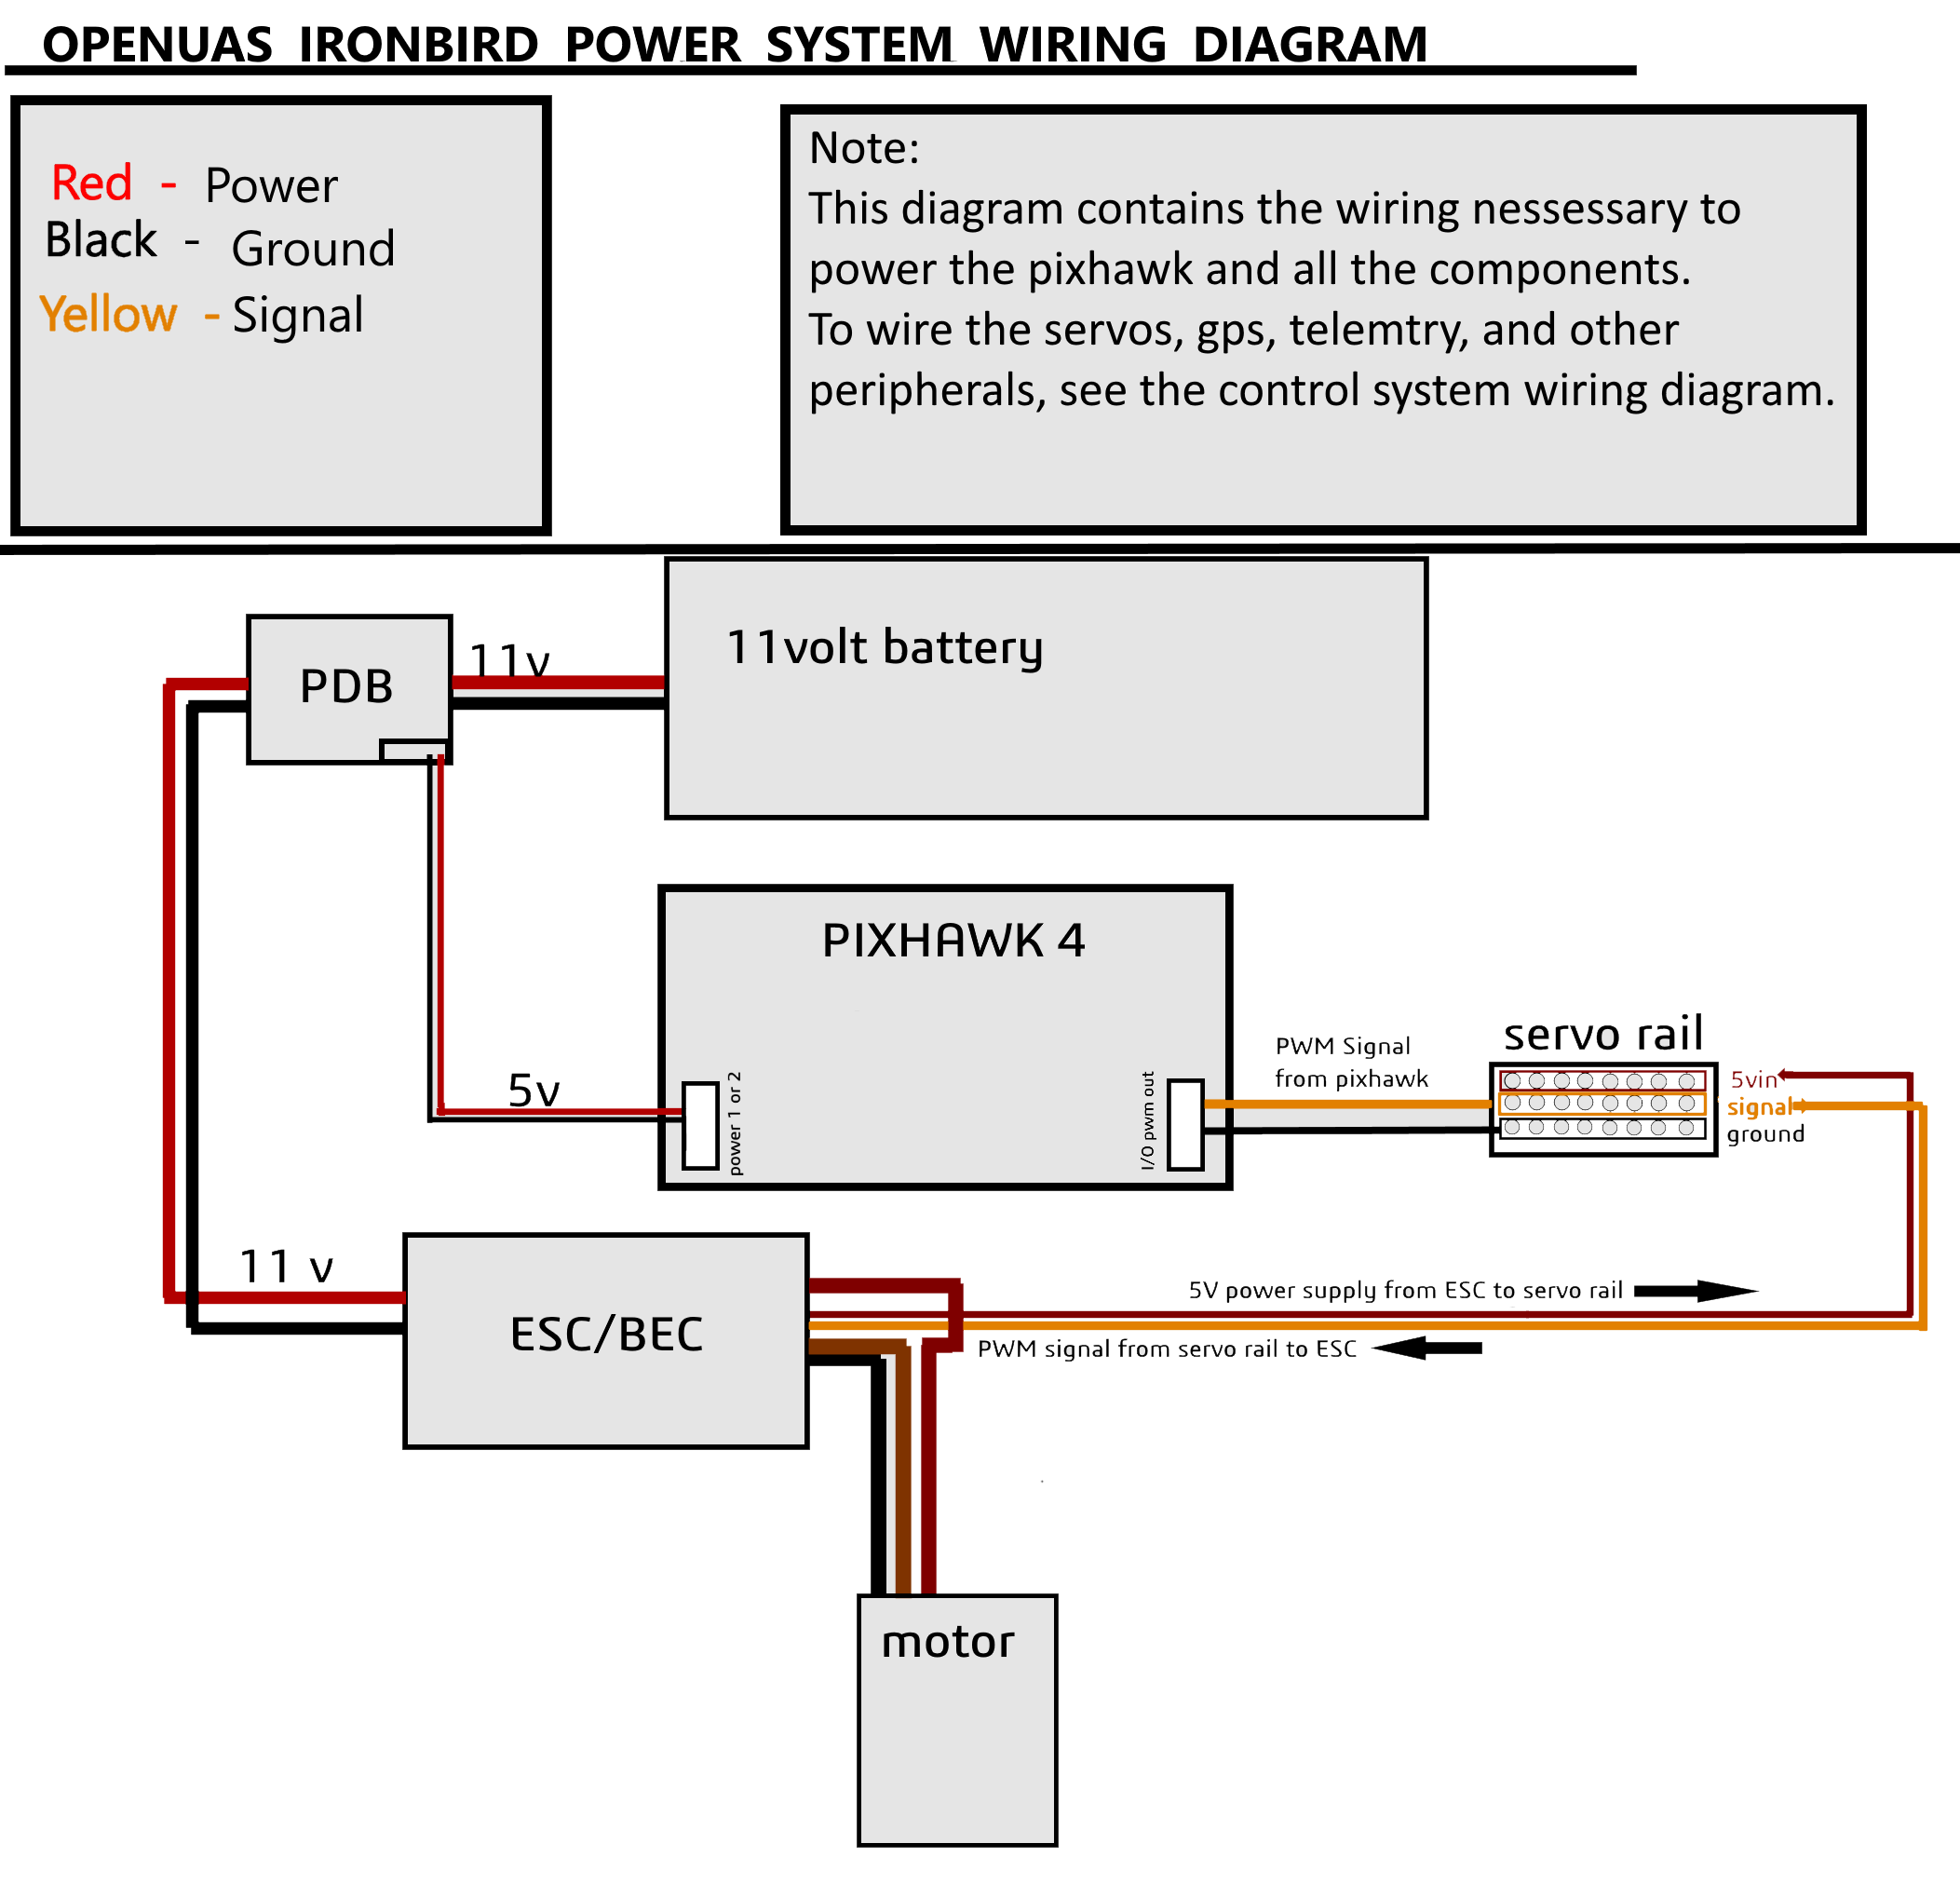
\includegraphics[width=0.8\linewidth]{Images/wiring powersyste v6.png}
\caption{Power System Wiring Diagram}
\label{fig:pwrsystm}
\end{subfigure}
\begin{subfigure}{0.5\textwidth}
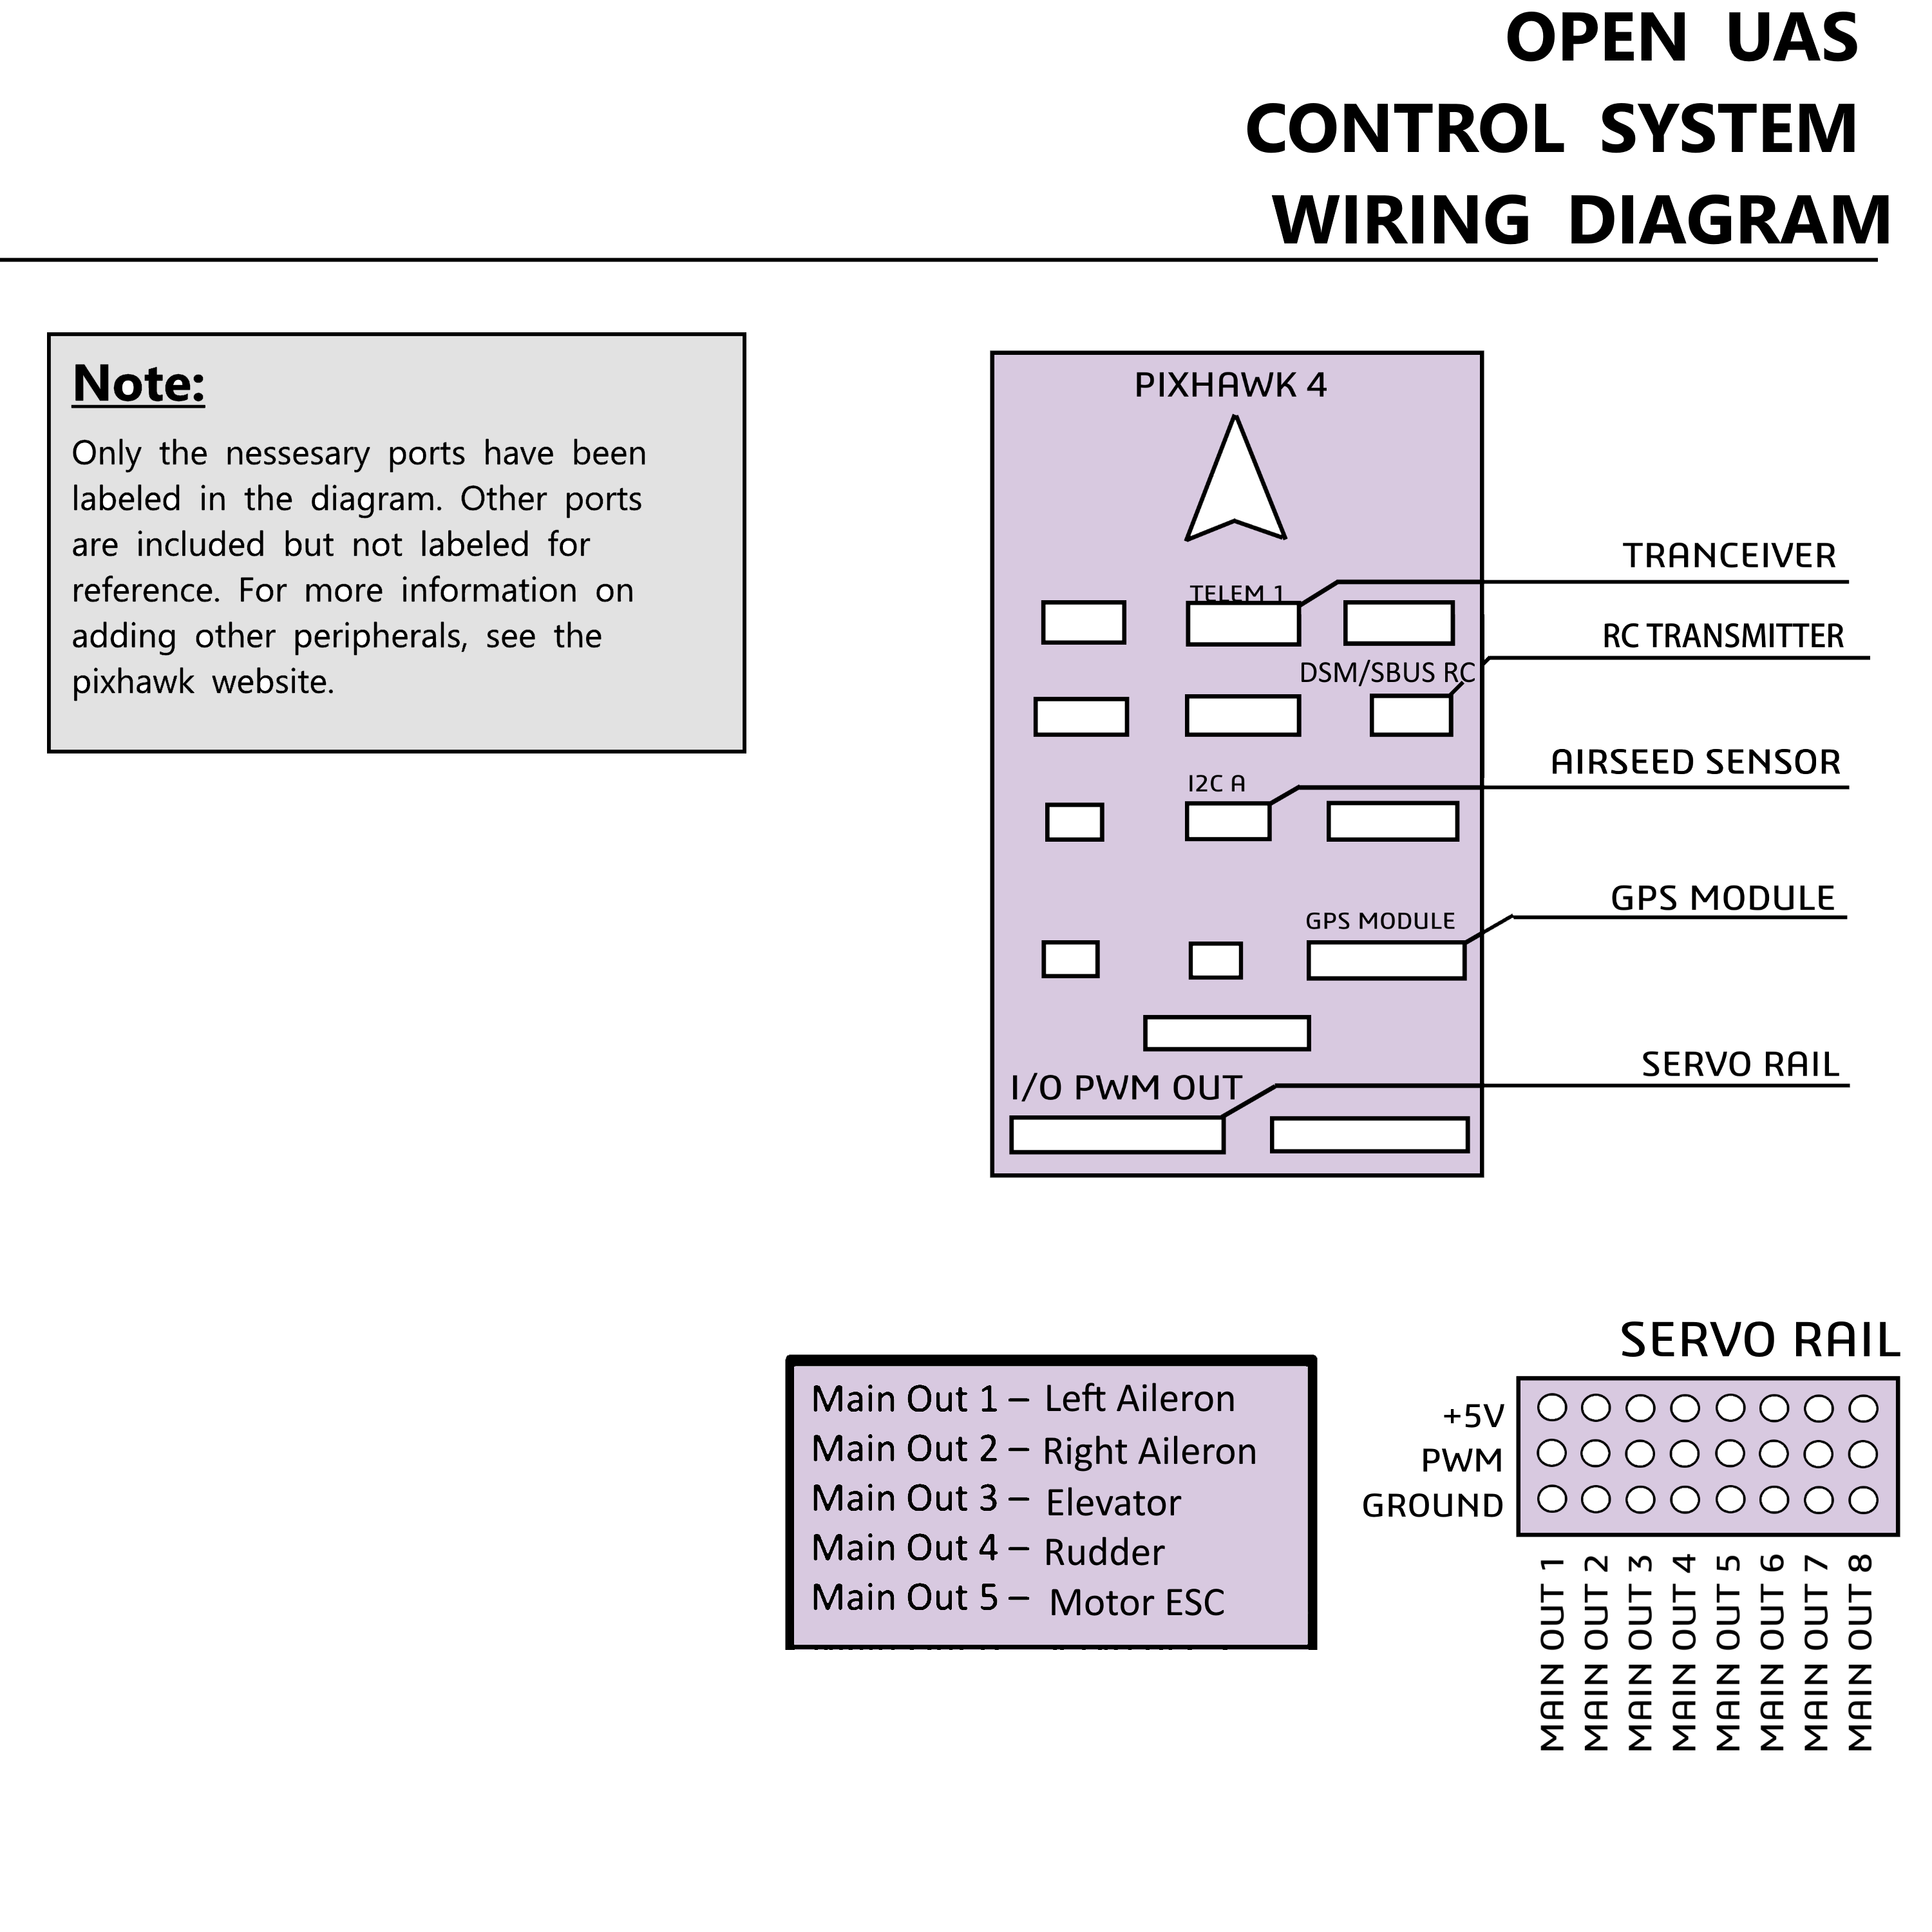
\includegraphics[width=0.75\linewidth]{Images/PIXHAWK4 control system wiring.png}
\caption{Control System Wiring diagram}
\label{fig:ctrlsystm}
\end{subfigure}
\caption{Wiring Diagrams}
\label{fig:wiringidagrsm}
\end{figure}
 \newpage
\paragraph{Motor \& Prop Selection}
To determine a motor and prop combination, and subsequently what ESC should be used, analysis was done using
data from both CFD and MotoCalc.
Every combination of motor and prop available in the lab was run via MotoCalc to generate theoretical values
for current draw, efficiency, and thrust available at varying velocities. The parasite drag coefficient
$C_{D,0}$ was found using data from CFD analysis run on the craft model and was used to find the thrust
required curve. A MATLAB script was written which compares data generated by MotoCalc using the thrust required
curve. The script and selection process were documented for future use. Along with $C_{D,0}$, the maximum lift
coefficient $C_{L_{max}}$ was found using CFD, and was used to compute the stall velocity, which came out to be
around 37 mph. This seemed high given the wing area of the craft, especially since the $C_{L_{max}}$ was around
.3, which is very low for $C_{L_{max}}$.\\

Ultimately the combination with the largest excess thrust was selected over valid combinations with higher efficiencies and lower current draws. This was due to the high calculated stall velocity and past flight tests where the UAS did not have enough thrust and crashed, so the team wanted to ensure that thrust would not be any issue during a test flight. The combination selected was a BadAss 3520-970Kv brushless motor in combination with an APC 15x8 prop. At 0 mph the MotoCalc calculated the maximum current draw to be 70 amps, and the current draw in steady state flight at 7 amps. The Badass Renegade 85A ESC was therefore chosen due to it's 85 amp continuous current draw and 100 amp burst current draw ratings.

%
\paragraph{Thrust Testing}
After manufacturing finished the UAS 2.0 body, the electronics team ran a standing thrust test to ensure the Iron Bird could sustain 100\% power without overheating issues. On November 21, 2020 we built a simple test stand in the lab to hold the UAS in place while the propeller was spun up, see figure~\ref{fig:standingThrustStand}. The UAS was enabled and the initial test was at very low power to ensure the propeller was spinning in the correct direction. Subsequent tests slowly increased the throttle and held it at 100\%. The total test time was $\sim$3 minutes. Shortly after the test we measured the casing of the motor and ESC with an infrared thermometer. The motor measured $\sim$100\degree F and the ESC was $\sim$120\degree F, both acceptable temperatures when considering the lack of airflow over the craft during this test. Unfortunately, the Pixhawk did not automatically log data during this test because there was no takeoff detected. The thrust produced during this test was not measured directly but from visual and auditory observation, appeared sufficient for flight. Overall the standing thrust test was a success and demonstrated that this Iron Bird configuration was capable of sustained flight without major issues.

\begin{figure}[!h]
    \centering
    \includegraphics[width=0.9\linewidth]{Images/standing_thrust_test1.jpg}
    \caption{Standing Thrust Test Setup}
    \label{fig:standingThrustStand}
\end{figure}


\subsubsection{Software}
\paragraph{Controls Mixing}\label{mixing}
The previous UAS design required two separate servos to control the elevators. This was not a setting that was available through the current airframe, and it required creating a more advanced mix on the Taranis controller as well as the use of one of the AUX PWM outputs. This meant that if any  flight mode other than manual was used, the Pixhawk would not "know" that the aux output was one of it's elevators and so it would not send control signals to the elevators in assisted and autonomous flight modes. The setup for flaperons had similar issues as well.

To remedy this problem, a custom controller mixer was written and placed on the MicroSD card in the Pixhawk 4, which overrides the current mixer for the Bormatec Maja airframe. The mixer allows for the customization of PWM outputs on the breakout board by mapping inputs from the control groups in the Pixhawk flight computer to the PWM out channels. This allows for the simplification of the electronics setup; it simplified wiring so only one PWM breakout Board was needed, simplified the mix on the Taranis flight controller, and allowed for the adjustment of the servo actuation direction and magnitude without modifying parameters in QGroundControl. This also meant it that we could test other flight modes, which are written about in sections~\ref{apprenticeflight} and~\ref{UASflighttest}. In future semesters, we hope to compile our own airframe with these changes such that the additional mix file will not be needed.

\paragraph{Flight Simulation}\label{simulation}
With the change to the new Pixhawk 4 this semester also came some experimentation into simulated test flights. The latest Pixhawk firmware allows for fully simulated flights using Gazebo to simulate the world that the software interacts with. Instead of QGroundControl connecting to the Pixhawk hardware over radio, it connects to a version of the Pixhawk firmware running locally on a lab computer. From there, the Pixhawk firmware communicates with Gazebo, also running locally on a lab computer, to interact with the simulated world.

We were able to run basic flight simulation tests of manual and some autonomous flight modes. We are currently using a default fixed-wing airframe for the simulations. We plan to add our own UAS design to the simulator to more accurately simulate the flight during the winter break. In the future, this system will allow us to train new pilots as well as test new software features. The simulation will give us a general idea of how the real UAS will behave without fear of crashing. This will also speed up development as the software sub-team will not have to wait for manufacturing to start testing flight modes.

We also explored hardware in the loop (HITL) simulation. QGroundControl connects to the Pixhawk hardware as usual over radio, but the Pixhawk sends commands and receives results from a simulated world running on a lab computer. This would integrate the flight hardware into the testing structure. However, HITL simulation is no longer supported by Pixhawk for fixed-wing aircraft. It was ultimately determined that HITL simulation did not provide a significant advantage over a standard full simulation composition for the amount of additional work required due to the dropped support.

\subsection{Flight Test Team}
The Flight Test team this semester performed two successful test flights of two different aircraft at a Radio Controlled (RC) aircraft flying field. Updated test plan templates for ground and flight tests were created and filled out for all test flights. Also, a document containing overall flight test outlines and objectives was created to specify the goals of flight tests for each aircraft from the flight test and electronics team's perspectives.

To perform test flights, the OpenUAS team needs access to a large open space with an improved surface to launch and recover aircraft from, more than 5 miles away from the Ames Municipal Airport. This need led the team to seek the use of the Central Iowa Aeromodelers flying field located South East of Ames Iowa. To obtain use of this field the team pilot needed to be a member of the Central Iowa Aeromodelers club and the Academy of Model Aeronautics (AMA), which was eventually received during the semester. Documents were also created that listed contacts and information gained this semester on the AMA and Central Iowa Aeromodelers, so future team members will know where to start when trying to obtain or renew a membership. Alternative membership options are also listed on these documents as well.


\subsubsection{Apprentice Flight Test}\label{apprenticeflight}
At the beginning of the semester, the new Apprentice trainer aircraft the team purchased last semester was assembled and readied to test out autonomous flight modes on the Pixhawk. Only minor modifications were required to integrate the necessary electronics. The main objectives for the initial Apprentice flight were to complete all maneuvers normal to flight, ensure control centers are in the correct place so the aircraft can cruise "hands-off," check control deflections, and perform several autonomous functions. Autonomous flight modes included Stabilize, Position, Hold, Return, and Mission.

\begin{figure}[!h]
    \centering
    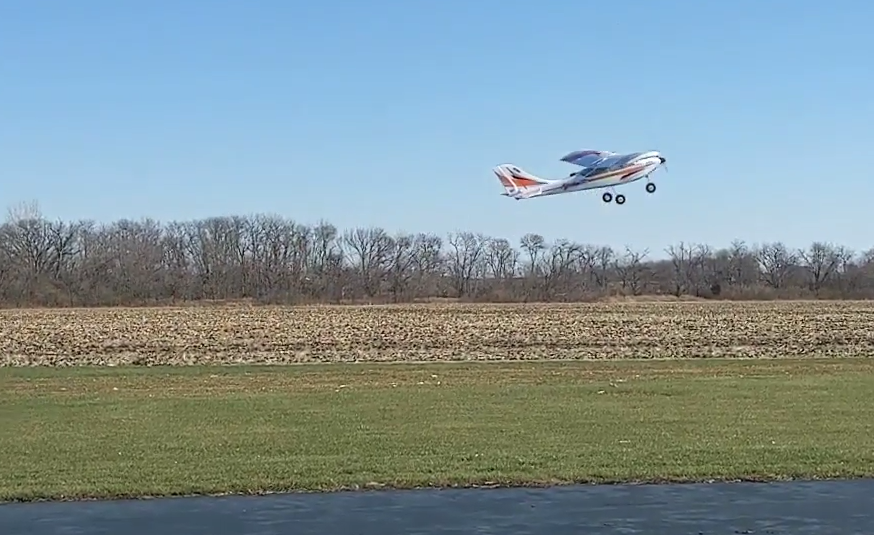
\includegraphics[width=0.9\linewidth]{Images/RANGER1.PNG}
    \caption{E-flight Apprentice in Flight}
    \label{fig:Rangertest}
\end{figure}


The Apprentice test flight occurred on November 13th, 2020 at the Central Iowa Aeromodelers flying field. Weather conditions were mostly nominal, with unlimited visibility and clear skies, the wind was out of the south (straight down the runway), but at a gusty 7-10 mph. The first flight was uneventful with the exception that it took all available nose-down trim plus a small amount of constant forward stick pressure to keep the nose of the aircraft level in cruise flight. This was attributed to an aft center of gravity (CG) condition, which will be corrected in the future with more strategic electronics placement. However, the slightly aft CG did not adversely affect the flight characteristics of the aircraft so the elevator center was adjusted down after the first flight and we proceeded with autonomous tests.

\paragraph{Flight Analysis}`Stabilize, Position, Hold, and Return tests went almost flawlessly and the aircraft was able to accurately correct for wind drift. The only flaw was that manual control deflections were greatly reduced in the Stabilize and Position modes, which the electronics team will look into fixing in the future. The Mission flight mode did not appear to follow waypoints closely and appeared to attempt to land the aircraft on its own so the aircraft was returned to manual control. A wind gust on the final landing caused a bounce and flipped the aircraft upside-down right above the runway, however, the only damage to the aircraft was the main landing gear coming loose, which can be easily repaired. Overall the first apprentice test flight was a resounding success, and the team gained a large amount of valuable flight data from the Pixhawk, as well as a confirmation that Pixhawk autonomous flight modes work well.


\subsubsection{OpenUAS Flight Test}\label{UASflighttest}
The first flight of the UAS 2.0, designed in the Spring 2020 semester, occurred on November 22nd, 2020 at the Central Iowa Aeromodelers flying field. Weather conditions were unlimited visibility and clear skies, the wind was out of the West at a gusty 7-10 mph. Once the preflight checks were completed the UAS was sat onto the carrier on the launch rail, and the team quickly determined that it was not sufficiently stable as the wings of the UAS would not stay level on their own and would likely hit the crossbar at the front of the launch rail on takeoff. The carrier had been completed that morning, so we had not had a chance to test it before the flight attempt. However, with the positive results of the thrust test in mind, the team determined that the UAS most likely had enough thrust for a hand launch to be successful. The UAS was powered up to full throttle as a team member ran with it, giving it a forward push as he let go, which was enough for the UAS to gain flying airspeed with little to no dip in flight path after release.
\begin{figure}[!h]
    \centering
    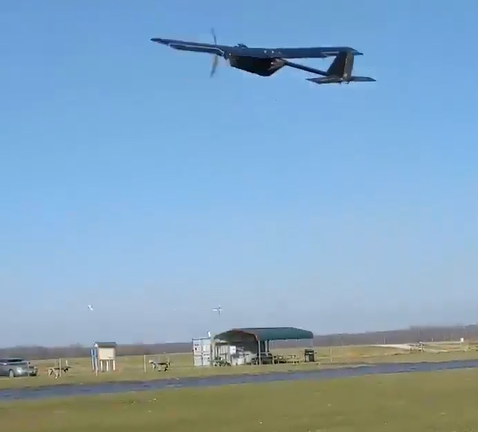
\includegraphics[width=0.5\linewidth]{Images/UAS1.PNG}
    \caption{UAS Version 2.0 in Flight}
    \label{fig:UASflight}
\end{figure}


In the air, the UAS was somewhat unstable, though not more so than many aerobatic RC aircraft. The flight controls were effective, though the ailerons were more effective than is necessary, and the rudder could use to be more effective. The UAS climbed very well and would cruise comfortably at around 75 percent power. Engaging the Stabilize mode effectively eliminated all stability problems and made the UAS as easy to fly as the Apprentice trainer aircraft. Flaperons (drooping ailerons to act like flaps) were tested and seemed to reduce the slowest possible flying speed of the UAS, as expected. A low battery warning occurred halfway into the flight but went away when the throttle setting was reduced to zero, so we determined that we could continue flying. However, not long after a wind gust hit the UAS in the middle of a turn, which sharply decreased the turn radius and stalled the inner wing causing a spin. Corrections to recover from the spin were immediately input (throttle cut, ailerons neutral, opposite rudder to the direction of the spin, and down elevator to break the stall), however, those did not work. Blips of power were also attempted but to no effect. At the last second the UAS was put into a flat spin (throttle cut, full ailerons opposite to the spin direction, and full up elevator) to slow its descent as much as possible for impact. The UAS hit the ground in a flat spin, but incurred fairly minor damage, with only one wing broke at a connection point and aileron hinges detached.

\paragraph{Flight Analysis}Reviewing the log data from the flight, the average ground speed was 36.6 mph with a peak of 73.5 mph shortly after takeoff. Looking at airspeed, the UAS flew at a peak airspeed of 53.7 mph at it slowest flew $\sim$33 mph. This was lower than the theoretical stall velocity, and was achieved without use of the flaperons. It is unclear whether this is the actual stall velocity or if the craft can fly slower, therefore further flight tests would be useful to determine this as well as to validate or invalidate the CFD. Additionally, we noticed that the Pixhawk reported a peak of 120 amps of current draw during takeoff and when attempting to recover from the spin. This about 1.4 times the max current draw that MotoCalc predicted. Upon investigation it seems like this is due to using the least accurate method of battery estimation, the same issue that likely caused the low battery warnings. However, at no time during the flight did we lose control or notice a reduction of power, and after the flight, the battery was measured to be above 11 volts, or 3.7 volts per cell which means there was still a safe amount of charge left. We plan to re-configure the Pixhawk to more accurately measure battery usage and further understand how it measures battery level.

Overall the first UAS flight was a success, as it was the first OpenUAS team designed aircraft to fly, and the damages from the crash will be easily repairable. The OpenUAS team learned a lot from what did and did not go well on this flight, and will work to make improvements and modifications to the UAS  2.0 design in the next semester, such as researching and implementing changes to improve aircraft spin recovery. Lessons learned from this flight will also be incorporated into the UAS 3.0 design created this semester, which we plan to build and possibly fly by the end of next semester.


%%LESSONS LEARNED%%
\section{Lessons Learned}

\begin{enumerate}
\item Start the semester with clear objectives, a practical timeline, and organized deliverables
\item UAS 2.0 is lighter than UAS 1.0, but still heavier than we would like. Our weight reduction measures worked, but we need to continue to implement more weight reduction in the future
\item UAS 2.0 is not as stable as we would like it to be
\item UAS 2.0 can not be recovered from a spin with reasonable altitude loss; potential design changes would be to increase rudder size as well as add rudder below the horizontal stabilizer
\item Building an aircraft in a rush to meet a deadline is less than ideal, and does not result in the highest possible build quality.
\item It is beneficial to have an understanding of the inventory in the lab; spare components that may be useful could be hidden away somewhere
\item While in the design process, constantly verify ease of manufacturing
\item The more details that can be included in the CAD model the better. \item More thought needs to be given to manufacturability and method of attaching components in the design process
\item Unplug the battery when plugging other components in
\item CFD is a useful tool, however it is not a crutch, and may not be accurate

\end{enumerate}

%%LIST OF FUTURE TASKS%%
\section{Future Tasks \& Deliverables}

\begin{itemize}
\item{Investigate Battery/Current Draw Readings}
\item{Run a Standing Thrust test to directly measure current Draw}
\item Repair Apprentice landing gear
\item Re-arrange electronics to move Apprentice CG farther forward
\item Continue to test Mission flights with the Apprentice
\item Repair and make improvements to UAS 2.0
\item Continue to test fly UAS 2.0
\item Validate or invalidate CFD run on UAS 2.0
\item Re-design and test launch rail
\item Complete OpenUAS design 3.0, taking into account lessons learned from UAS 2.0
\item Test fly OpenUAS design 3.0
\item Investigate the possibility of a 3D printed airframe,simliar to designs seen here: \hyperlink{https://3dlabprint.com/shop/}{https://3dlabprint.com/shop/}
\end{itemize}


%%REFERENCES%%
\unlabeledsection{References}

\end{document}
